\mysubsectionformatted{Design Pattern State}
\myparagraph{

    \begin{tcolorbox}[colback=blue!5!white, colframe=blue!75!black]
        Permette a un oggetto di modificare il suo comportamento quando il suo
        stato interno cambia.
    \end{tcolorbox}

    \noindent\textit{State} viene utilizzato quando si vuole modificare lo stato interno di un oggetto
    in modo da potergli far eseguire determinati metodi. Gli stati degli oggetti vengono rappresentati
    da classi differenti che estendono una classe astratta che rappresenta lo stato dell'oggetto.

    \begin{center}
        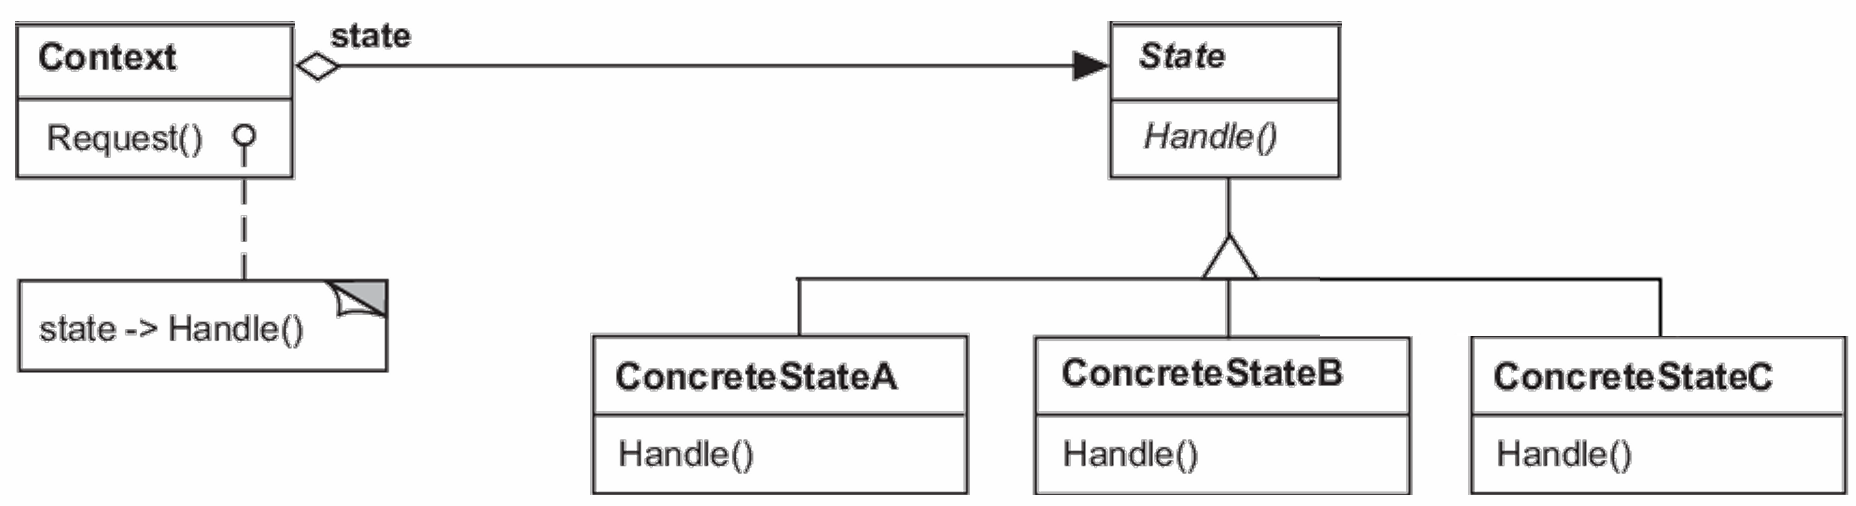
\includegraphics[scale=0.25]{Esercitazione - Design Patterns/state_pattern.png}
    \end{center}

    \begin{enumerate}
        \item \textbf{Context} è l'interfaccia del client. Ha un'istanza di \textbf{ConcreteState} che indica in che stato si trova.
        \item \textbf{\textit{State}} è la classe astratta che rappresenta lo stato attuale di \textbf{Context}.
        \item \textbf{ConcreteState} sono le classi che implementano il comportamento \\associato allo stato del \textbf{Context}.
    \end{enumerate}

    \begin{center}
        \resizebox{\columnwidth}{!}{%
            \begin{tabular}{|l|l}
                \hline
                \rowcolor[HTML]{32CB00}
                \multicolumn{1}{|c|}{\cellcolor[HTML]{32CB00}\textbf{Vantaggi}}                                                                       & \multicolumn{1}{c|}{\cellcolor[HTML]{FE0000}\textbf{Svantaggi}} \\ \hline
                Eliminazione di tanti "if"                                                                                                            & \multicolumn{1}{l|}{Incremento del numero di oggetti}           \\ \hline
                Facile lettura del codice                                                                                                             & \multicolumn{1}{l|}{Richiede la scrittura di molto codice}      \\ \hline
                \begin{tabular}[c]{@{}l@{}}Nuovi stati e transizioni possono essere\\ aggiunti facilmente definendo nuove \\ sottoclassi\end{tabular} &                                                                 \\ \cline{1-1}
            \end{tabular}%
        }
    \end{center}

    \newpage
    \subsubsection{Esempio di Pattern State}
    \begin{center}
        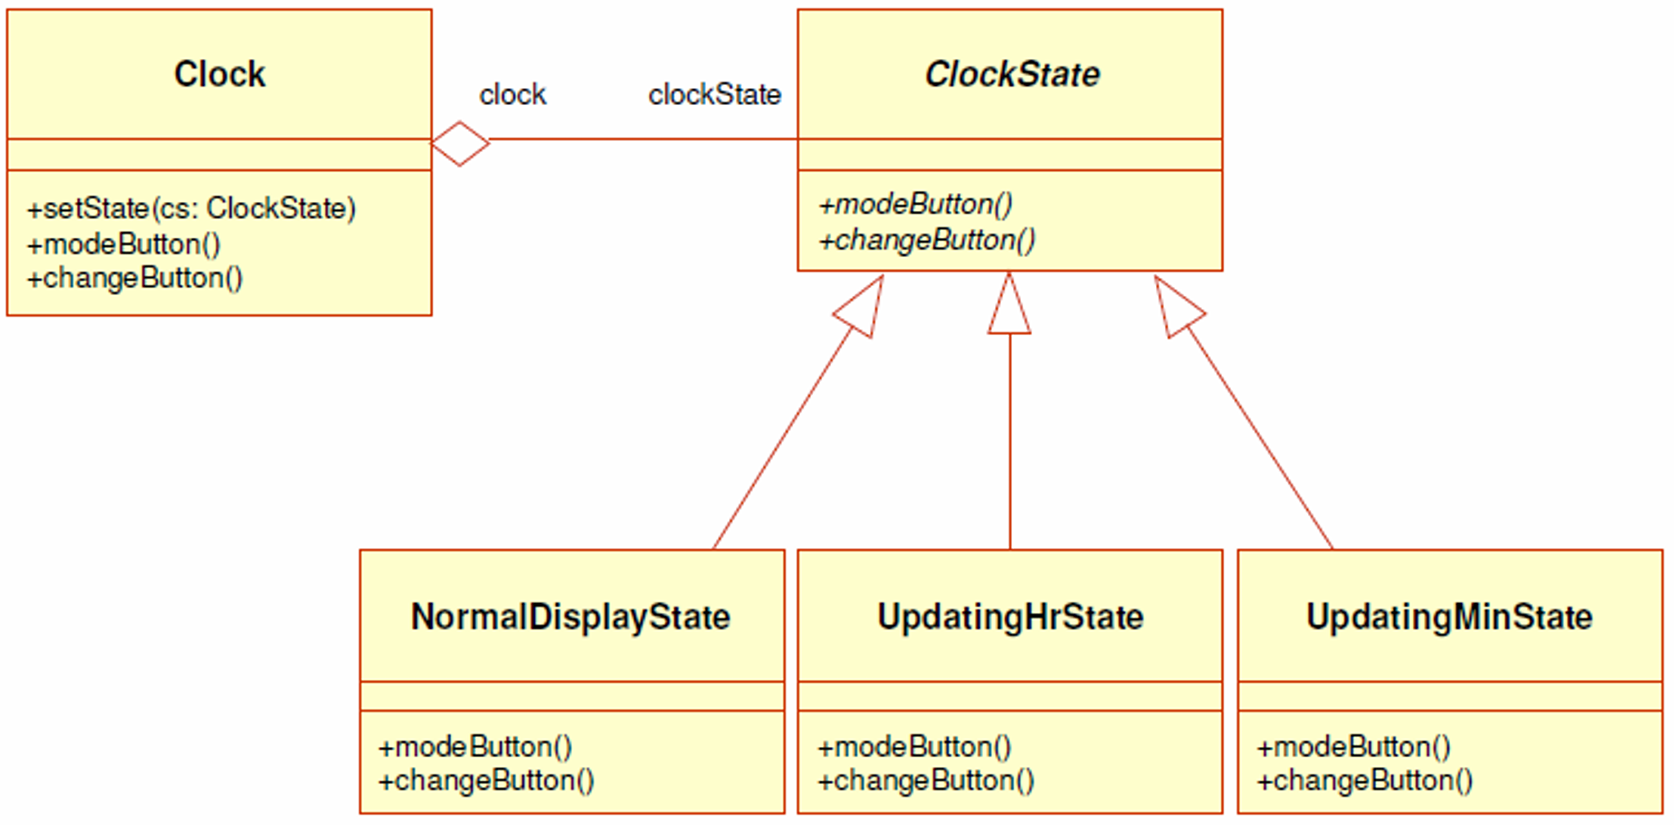
\includegraphics[scale=0.25]{Esercitazione - Design Patterns/example_state_pattern.png}
    \end{center}
    In questo esempio, \textbf{Clock} contiene 3 metodi di cui \textbf{modeButton()} e \textbf{changeButton()} cambiano il loro
    comportamento in base allo stato in cui si trova. \textbf{setState(cs: ClockState)} permette di cambiare lo stato di \textbf{Clock},
    in questo modo, anche i due metodi all'interno cambieranno il loro comportamento.

    \mysubsubsectionformatted{State vs Strategy}
    Sono entrambi pattern comportamentali, ma hanno obiettivi e applicazioni \\differenti.

    \begin{tcolorbox}[colback=blue!5!white, colframe=blue!75!black]
        State cambia il comportamento di un oggetto in base al suo stato interno.
        \\Es. Un lettore audio che può avere stati come "Play", "Pause" e "Stop", dove ogni stato 
        gestisce le azioni dell'utente in modo diverso.
    \end{tcolorbox}

    \begin{tcolorbox}[colback=green!5!white, colframe=green!75!black]
        Strategy consente di cambiare il modo in cui un'operazione viene eseguita, senza modificare lo stato interno dell'oggetto.
        \\Es. Un sistema di pagamento che può usare diverse strategie come "Carta di credito", "PayPal" o "Bonifico", a seconda della scelta dell'utente.
    \end{tcolorbox}
    \newpage

}